
\textbf{Eu sou Eu} está a adorar a sua experiência no planeta Terra, aquela pinta cósmica, a qual também chamam de planeta Azul.

Mesmo sendo um planeta habitado por humanos, no geral, conflituosos, com os nervos à flor da pele, num rebuliço contínuo e uma boa dose de egoísmo, também existem seres pacíficos que vivem com tranquilidade, muita paciência e generosidade.

Neste mundo de 3ª dimensão, onde as formas têm volume e o tempo é linear, vive-se a dualidade onde os opostos estão presentes – bem e mal, feio e bonito, alto e baixo, frio e quente e por aí em diante.

Há muito, muito tempo mesmo, o conjunto da humanidade desligou-se da Fonte que lhe deu Vida, esquecendo o Pai Criador. E agora, os homens acordam todos os dias de manhã, colocam as tais máscaras, vestindo assim as suas personalidades e, num estado de sonambulismo, vivem uma ilusão pensando ser a Realidade.

Correm atrás do vento.

Eles esqueceram o que realmente é importante e que está dentro do coração: a Essência. E por essa razão, os homens creem-se separados, distantes uns dos outros. Umas vezes estão amigos e outras vezes estão zangados.

Possuir Sabedoria é ter consciência disso, respirando e aspirando regressar à Unidade.
\bigbreak
Gaia, a Mãe Terra, sempre conciliadora, alimenta, acolhe e dá proteção aos seus filhos. O seu manto é um colo carinhoso. Montanhas rochosas e altas dão espaço a vales serenos, florestas extensas e densas estão de mãos dadas com prados suaves, animais de grande porte partilham o território com os mais pequenos.

Os homens, esquecidos de que são todos irmãos e achando-se inteligentes, querem tudo para si.
Compram, vendem, roubam, apropriam-se do que é gerado pela Terra como dádiva e de uma forma generosa para todos.
\bigbreak
O Mundo é apenas um, mas, sem dúvida, que cada homem vive no mundo que constrói ao seu redor.
\bigbreak
\textbf{Eu sou Eu} prepara uma surpresa para os seus divertidos amigos.
\bigbreak
— Vamos dar uma volta? – pergunta.
\bigbreak
Não foi preciso esperar pela resposta.

Todos já estão alinhados com mestria, como pequenas abelhas dentro dos favos de uma colmeia.

\textbf{Eu sou Eu} ajusta a sua antena interplanetária com a mão esquerda, concentra-se por uns segundos e solta um sorriso gigante. Neste preciso momento contata com o seu mundo, AnThais, que lhe retribui o sorriso.

A colaboração na surpresa que \textbf{Eu sou Eu} resolveu ofertar, vem do seu planeta que está a 81 trilhões de quilômetros de distância da Terra.

No céu forma-se uma espécie de espiral de vento e centenas de Esferas Transdimensionais voam para junto do canteiro dos lírios.

Começam a sua descida e aterrissam com tanta precisão que ninguém tem necessidade de dar um passo para o lado.

A luz emitida por cada esfera transparente fusiona-se com cada inseto.

Estes sentem uma estranha Leveza e levitam em sincronia no ar.

Forma-se um redemoinho de bolas de sabão, que volitam novamente por todo o jardim.
\bigbreak
A menina com o cata-vento na mão apercebe-se da magia que envolve o espaço onde brinca e, sem questionar o que são aquelas bolas, corre e canta no meio delas.
\bigbreak
— Foquem no centro! Não se desalinhem! Juntos vamos longe e mais Além! – diz \textbf{Eu sou Eu}, sabendo que se fazia entender.
\bigbreak
O conjunto dos insetos está radiante.

Todos voam, mesmo os que não sabem voar.

A ET permite-lhes ir onde querem, bastando visualizar o destino e focar o tal centro.
O centro do seu Coração.

A nuvem das bolas galácticas ascende até às árvores e eles observam um fulgor intenso que nasce nas suas folhas vibrantes.

Não é só o reflexo do sol que as faz brilhar assim. Há algo mais naquelas árvores.

 \textbf{Eu sou Eu} entra em comunicação telepática com elas, e os insetos recebem também a mensagem.
 \bigbreak
— “Vocês são os pulmões deste mundo, AnThais contempla-vos com reverência”.
\bigbreak
E as árvores magnificentes, naquele momento, assumem-se como representantes do Reino Vegetal e inclinam-se com o vento, numa vénia, em cortesia ao viajante e à bicharada.
\bigbreak
\textbf{Eu sou Eu} transmite:
\bigbreak
— Se os humanos pudessem ter apenas um pinguinho de perceção do que a Natureza sente com os seus atos e hábitos, ficariam envergonhados. Devastam florestas, queimam e arrasam bosques. As árvores, que tudo observam no silêncio, nunca perdem a atitude, mantendo as suas raízes firmes na terra e o seu tronco direito, porque são extremamente conscientes. Elas unem a Terra ao Céu.
\bigbreak
As plantas, as flores, todo o Reino Vegetal, são portais de consciência.

Consciência é Vibração. A Vibração é Luz. E a Luz, neste Reino tão extenso que se doa com Amor, transpira uma beleza sem limites e assume formas bem definidas, gerando sensações de cor, de aroma e sabor a quem sabe apreciá-las.
\bigbreak
— Eu, às vezes, como umas folhinhas das árvores. – diz baixinho uma lagarta gorda.
\textbf{Eu sou Eu} sorri. Pilota a sua ET para junto da ET da lagarta que falou, e diz:
\bigbreak
— E elas agradecem-te, porque ajudas na sua transformação e permites que folhas novas cresçam. E depois de muito comeres, entras também em TRANSFORMAÇÃO! Procuras abrigo nos seus ramos verdes, teces um delicado casulo e, dentro desse útero de seda, implodes em Metamorfose, renascendo em Borboleta. Assim, adquires a liberdade de voar para onde quiseres. Olhem só que mundo louco!

— É verdade, passo da Terra para o Ar. Desapareço numa forma e reapareço noutra ainda mais bela. Transito entre dois mundos diferentes, sem ter que sair deste mundo.
\bigbreak
E não são só as lagartas que vivem a Metamorfose.

A Vida é Metamorfose, Transmutação, Mudança.
O movimento não pára.

O verão sucede à primavera.

A noite vem depois do dia.

Enquanto uns dormem outros despertam.
\bigbreak
Os humanos que habitam a Terra, e estão unidos pelo Coração, sentem-se como irmãos.

Acenderam uma Luz no seu peito, como uns faróis na escuridão.

Têm Consciência de Si, vivem a verdadeira Liberdade em seus pensamentos e atos, têm uma enorme Responsabilidade para com a Terra-Mãe.

Acordaram do tal sonambulismo que ainda envolve grande parte da humanidade.

Os humanos, que são conscientes e lúcidos, embriagam-se na Natureza com a Simplicidade de uma flor, envolvem-se nela com a Humildade de uma gota de chuva e são Transparentes como um cristal, que deixa passar a luz.

Todos os seres conscientes e lúcidos conseguem transcender o que é imperceptível; a Vida flui para eles e a Natureza retribui-lhes, sempre!
As crianças sabem fazê-lo melhor do que ninguém.
\bigbreak
Se esta humanidade tomasse consciência da Força destas palavras, do seu Poder invisível e as vivenciasse, um Mundo Novo renasceria.
\bigbreak
M E T A M O R F O S E A R –S E–I A!
\bigbreak
Os insetos dão lições aos humanos, se estes quiserem apreender.
\bigbreak
— Vamos para junto das pedras! – \textbf{Eu sou Eu} assobia a toda a “frota galáctica”.
\bigbreak
Numa formação perfeita, deslocam-se para um riacho perto da casa do jardim.

Pedregulhos, pedras e pedrinhas cristalinas, com muitos tons e feitios, beijam amorosamente a água do riacho que corre com rebeldia e frescura.

As pedras pressentem a sua chegada e reluzem em Alegria. Elas são a Alegria.

Uma onda de Energia paira sobre o local. Vinda de cima e do chão. Vinda do Nada. Essa Energia é Consciência.
\bigbreak
— Vejam como as rochas são bonitas e brilhantes!
\bigbreak
\textbf{Eu sou Eu} faz um voo rasante ás pedras e os insetos seguem-no em fila indiana.

Alguns tocam-nas e as pedras vibram, sentindo-se afagadas.
\bigbreak
O Reino Mineral é o alicerce do mundo. Ampara com solidez as construções da Natureza, fortifica os lugares deixando-os em liberdade. E igualmente, doa-se num Amor livre, selvagem, estático e capaz de provocar o êxtase.

Este reino é Uno, onde tudo simplesmente É!

O Reino Mineral é puro Amor!

A viagem nas ETs oferece um oásis de prazer. Os insetos do jardim riem tanto dentro das bolas que as fazem rebolear.

A terra vista do céu numa perspetiva ampla, apresenta-se com padrões, esboços e desenhos perfeitos que se entrelaçam e complementam.
A Mãe Natureza é pintora e escultora.

Com o verde das plantas pincela o castanho da terra, com o azul da água lambuza a cor cinza das pedras. Espalha flores multicores por todo o seu tecido, jogando-as ao vento. E finaliza a sua tela com salpicos de animais e bandos de aves que não sossegam no mesmo lugar.
\bigbreak
— Vamos voar com os pássaros! – alguém diz e a concordância é global.
\bigbreak

\begin{figure}[h]
    \centering
    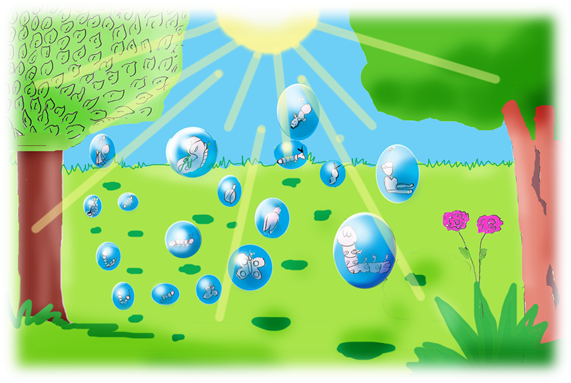
\includegraphics[width=0.85\textwidth]{bolhas}
\end{figure}

 Gera-se uma confusão no céu, é uma mistura de aves e Esferas Transdimensionais voando todas em bando. Ora sobem, descem, ora viram e rodopiam impregnadas de Alegria. Estão em Unidade. São a Unidade!
 \bigbreak
— Nunca voei tão rápido, vou ultrapassar uma andorinha. Que bom! – diz uma joaninha numa alegria efusiva.

— E eu nunca tinha voado, e as coisas lá em baixo, vistas daqui de cima, ainda são mais bonitas. – profere uma formiguinha.

— Estou enfeitiçado por esta ET, sinto-me leve como uma pluma! – diz a lagarta gorda, que achava que não cabia na “bola de sabão”.
\bigbreak
A viagem prossegue e o bando observa grupos de coelhos que saltam entre tufos de margaridas selvagens, um rebanho de ovelhas que pastam num prado verde, uma ninhada de patinhos que seguem a mãe pata e até passam por um enxame de abelhas apressadas para chegarem à colmeia, pois o dia está prestes a findar.
\bigbreak
\textbf{Eu sou Eu} comunga com a variedade de vida que não existe em AnThais, integrando-se na sua aura que está para além da visão - A Unidade do que é plural.
\bigbreak
\textbf{Eu sou Eu} diz aos insetos:
\bigbreak
— Vocês e todo o reino animal, têm forma e individualidade, mas, contrariamente aos homens, não sabem o que é a solidão, porque funcionam em grupo. O vosso corpo é separado dos demais, mas a vossa consciência é UNA. Por isso vivem em Paz com o que é natural.
\bigbreak
No Reino Animal, que não o homem, cada Ser respeita a natureza pelo que ela É, oferecendo-se em seu serviço. Ajudam-na a renovar-se sem perder o equilíbrio.

E do mesmo modo, a Mãe Natureza serve este Reino atendendo as suas necessidades.
\bigbreak
“Os pássaros não se preocupam com o que vão comer amanhã”.
\bigbreak
Utilizam-se, sem se usurparem. Agrupam-se, sem se aprisionarem.

Ninguém tira proveito de ninguém.

Têm uma relação de Simplicidade e de Amor!
\bigbreak
O dia voa como as aves e o sol começa a descer no céu.

A jornada pelos Reinos chega ao fim.

É tempo de regressarem ao jardim.

Sintonizam e sincronizam as ETs e elas embalam-nos de volta ao relvado.

Joana ainda brinca com o cata-vento.

Para ela o tempo não passou, e todos os relógios estão parados.
\bigbreak
Apenas o Sol desliza na quietude do céu azul, ofertando-se em Eternidade e em infinito Absoluto. Absoluto Amor, que é a referência para quem vive o que está dentro do seu Coração.
